\noindent \textred{3.} 
Build an AVL tree step by step. The keys are inserted in the order of:\{31, 20, 12, 26, 28, 27\}. Please draw the tree after each key is inserted, and mark the type of rotation taken, if any, at each step.

\noindent \begin{minipage}[t]{.24\textwidth}
    \vspace{0pt}
    \textblue{insert key 31;} \\ \\
    \centering
    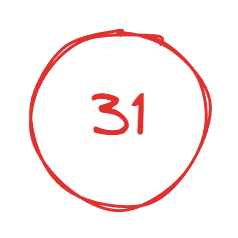
\includegraphics[width=0.36\linewidth]{HWs//HW7//figures/3_1.png}
\end{minipage}
\begin{minipage}[t]{.24\textwidth}
    \vspace{0pt}
    \textblue{insert key 20;} \\ \\
    \centering
    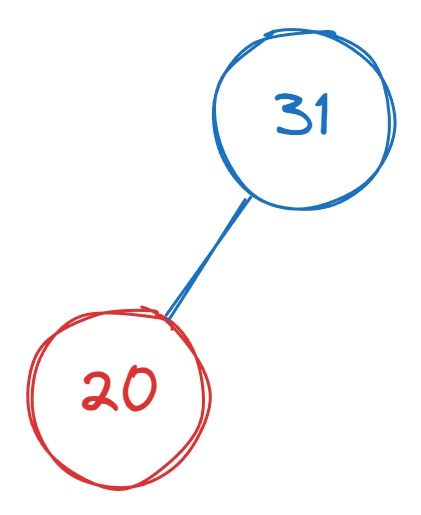
\includegraphics[width=0.65\linewidth]{HWs//HW7//figures/3_2.png}
\end{minipage}
\begin{minipage}[t]{.24\textwidth}
    \vspace{0pt}
    \textblue{insert key 12; \\(single rotation)} \\
    \centering
    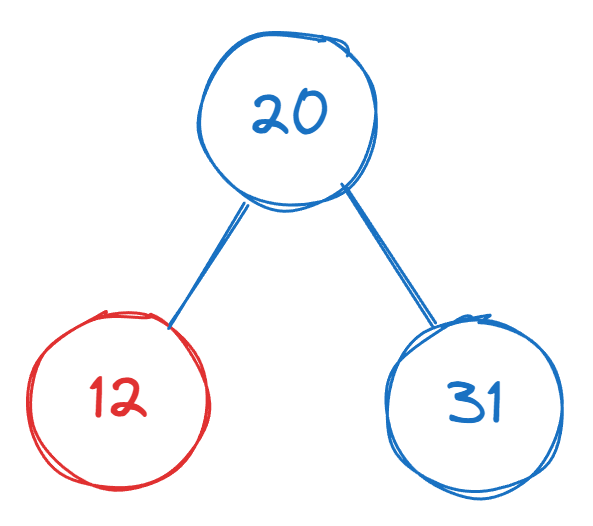
\includegraphics[width=0.88\linewidth]{HWs//HW7//figures/3_3.png}
\end{minipage}
\hspace{10pt}
\begin{minipage}[t]{.24\textwidth}
    \vspace{0pt}
    \textblue{insert key 26;} \\ \\
    \centering
    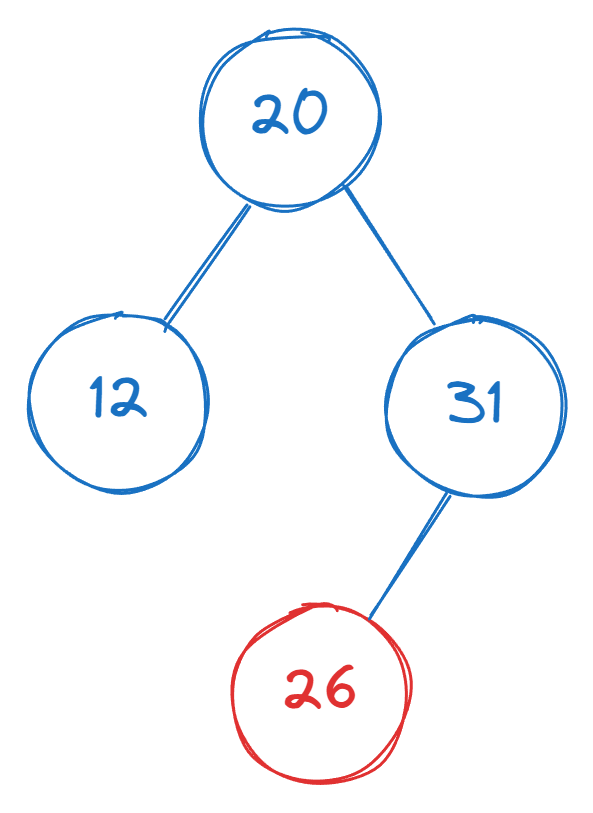
\includegraphics[width=0.88\linewidth]{HWs//HW7//figures/3_4.png}
\end{minipage}
\\ \\
\begin{minipage}[t]{.40\textwidth}
    \vspace{0pt}
    \textblue{insert key 28;\\(double rotation)} \\
    \centering
    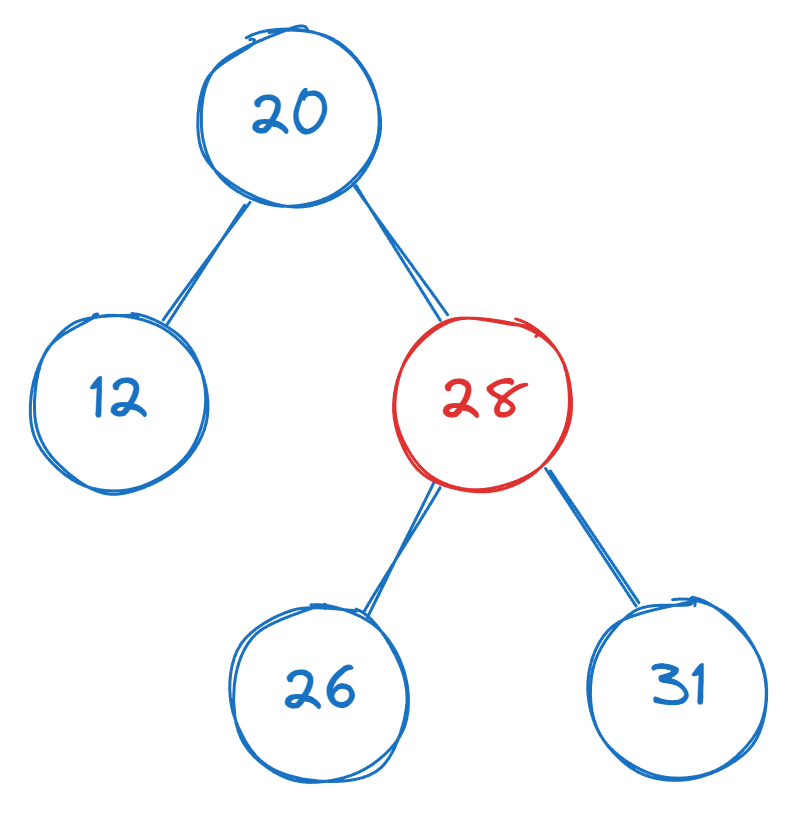
\includegraphics[width=0.73\linewidth]{HWs//HW7//figures/3_5.png}
\end{minipage}
\begin{minipage}[t]{.40\textwidth}
    \vspace{0pt}
    \textblue{insert key 27;\\(double rotation)} \\
    \centering
    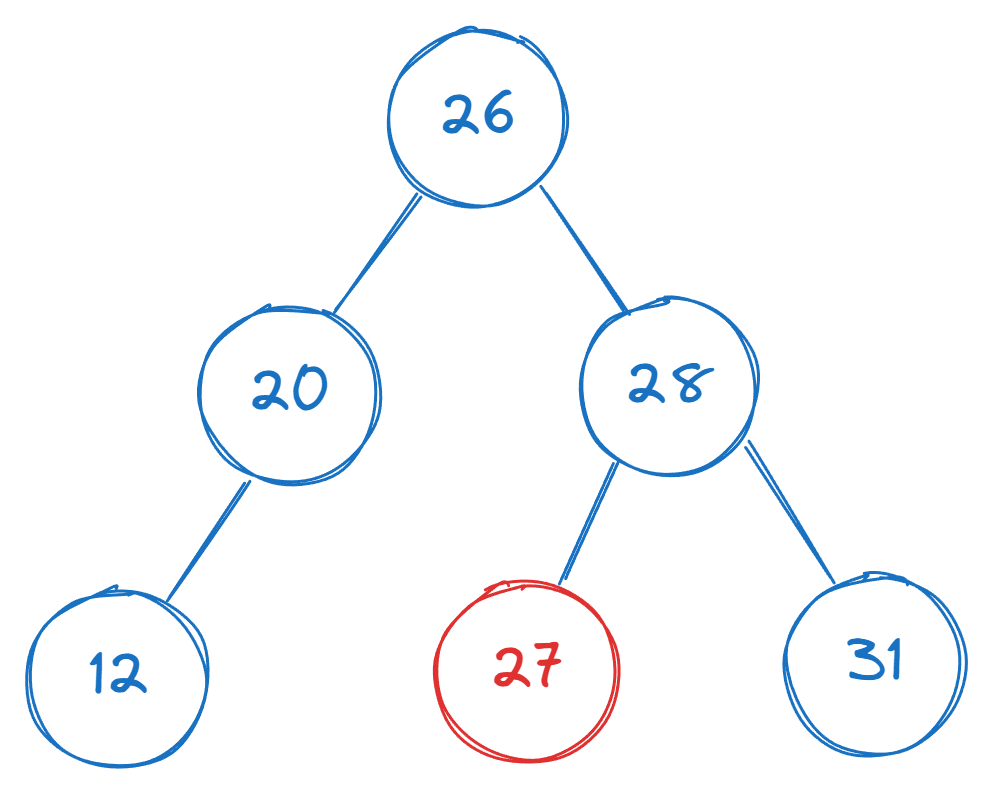
\includegraphics[width=0.93\linewidth]{HWs//HW7//figures/3_6.png}
\end{minipage}
